\chapter{Graphic User Interface}

\section{Serial Communication}

\begin{figure}
\centering
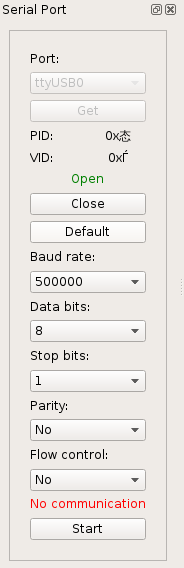
\includegraphics[width=0.3\textwidth]{images/gui/serial-port}
\end{figure}

\section{Logging}

\begin{figure}
\centering

\includegraphics[width=0.8\textwidth]{images/gui/logger}
\end{figure}

\section{Live Plotting}

\begin{figure}
\centering
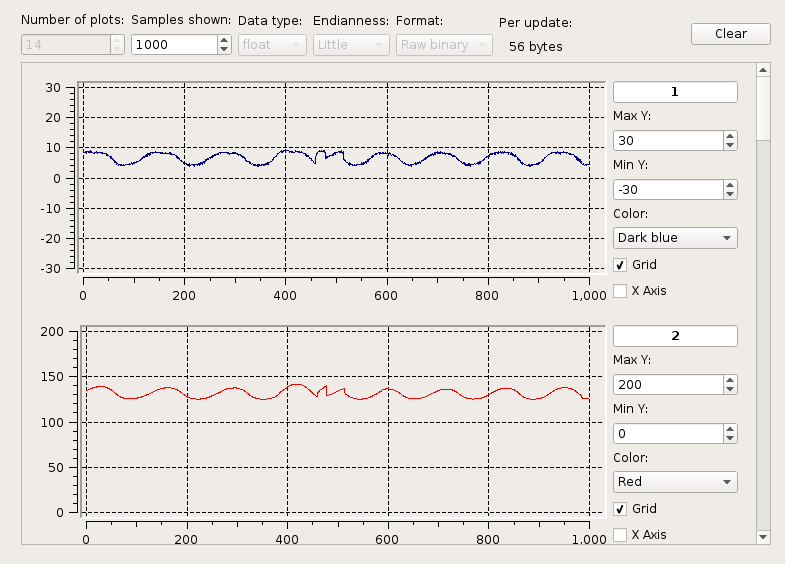
\includegraphics[width=0.7\textwidth]{images/gui/plotting}
\end{figure}

\section{Control Plug-in}

\begin{figure}
\centering
\subfloat[][Configuration \& On-board Control]{
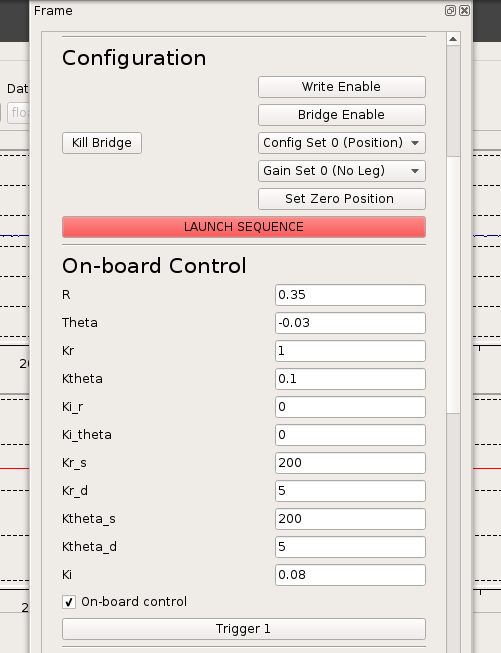
\includegraphics[width=0.4\textwidth]{images/gui/frame-1}
}
~
\subfloat[][Current/Position Control \& Control Loop Gains]{
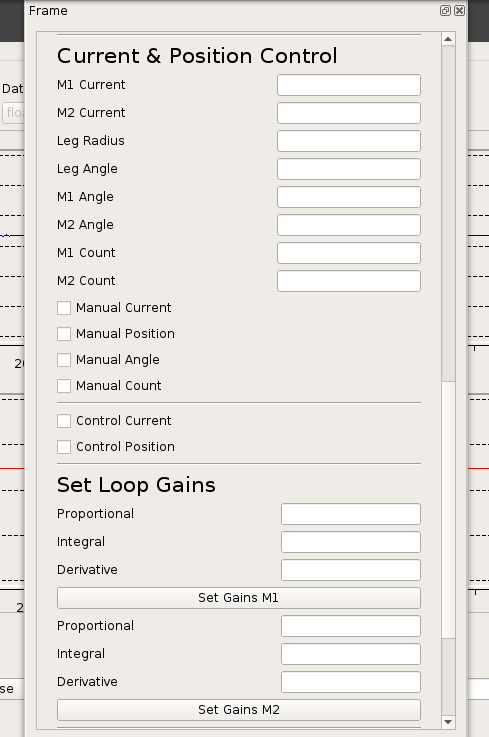
\includegraphics[width=0.4\textwidth]{images/gui/frame-2}
}
\caption{Control interface plug-in.}
\label{fig:Control interface plug-in} 
\end{figure}

